% ======================================================================
% col: 20

\chapter{Implementazione}
In questo capitolo verranno descritti i passaggi implementati per generare la raceline ottima data una
mappa.

Il lavoro svolto è stato basato sulla seguente repository GitHub:
\url{https://github.com/CL2-UWaterloo/Raceline-Optimization}.

\bigskip
\noindent I passaggi ad alto livello sono i seguenti:
\begin{enumerate}
	\item Ottenere l'immagine di una mappa (per esempio attraverso \hyperref[par:slam]{SLAM});
	\item Eventualmente ripurla di imperfezioni e ottenere un circuito chiuso; 
	\item Generare la centerline e calcolare la larghezza del circuito;
	\item Applicare gli algoritmi di generazione della raceline;
\end{enumerate}

%TODO:spiegare occupancy grid?
Operativamente, la mappa deve essere file in immagine che rappresenta una occupancy grid binaria, mentre
i percorsi, che siano raceline o centerline, sono in formato csv con almeno due colonne rappresentanti la
posizione $(x,y)$ di ogni sample e almeno una terza colonna per la velocità per quanto riguarda la
raceline. Successivamente si è scelto di esportare anche l'orientamento del robot rispetto alla mappa e
l'accelerazione per ogni sample.

\section{Generazione centeline}
Affinchè l'algoritmo per l'estrazione della linea di riferimento restituisca un risultato corretto, come
detto in precedenza, l'immagine della mappa deve rappresentare un circuito chiuso e con bordi ben
definiti e lisci, come effettivamente sarebbe un circuito di F1.
Dunque se si acquisice una mappa con SLAM come in figura \ref{fig:slam_map} è necessario modificarla come
in figura \ref{fig:slam_map_mod}. Durante l'implentazione di questa tesi si è deciso di usare le mappe
dei circuiti da gara più famosi forniti da F1TENTH stesso \cite{f1tenth-gitmaps}.

% TODO: cambiare dimensioni immagini (gimp)
\begin{figure}[H]
	\begin{minipage}[c]{0.5\textwidth}
		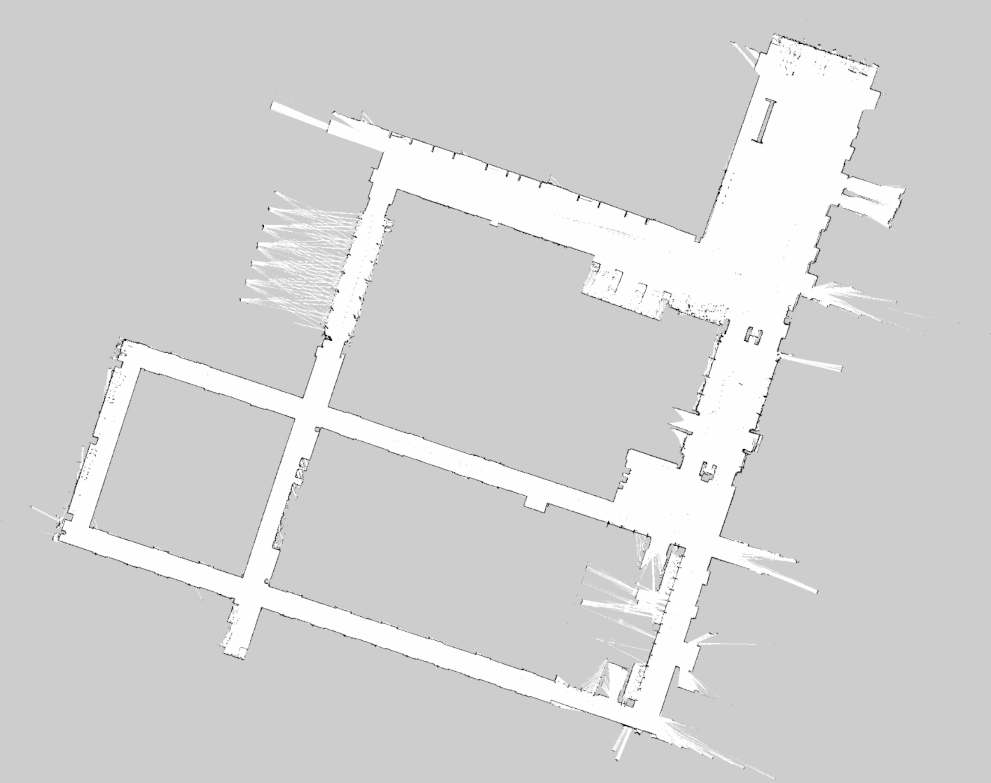
\includegraphics[width=0.9\textwidth]{slam_map.png}
		\caption{Comparazione tra raceline ottimale, in verde, e raceline geometrica, in blu tratteggiato}
		\label{fig:slam_map}
	\end{minipage}\hfill
	\begin{minipage}[c]{0.45\textwidth}
		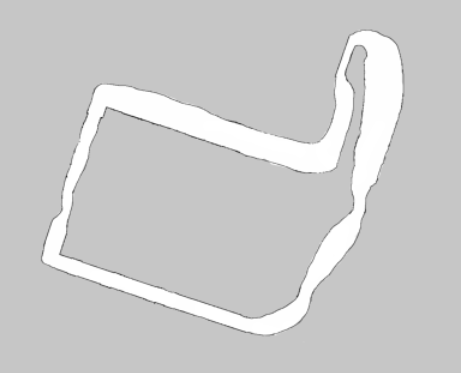
\includegraphics[width=1\textwidth]{slam_map_mod.png}
		\caption{Confronto tra raceline ottime con due curve distinte in sequenza}
		\label{fig:slam_map_mod}
	\end{minipage}
\end{figure}

